\chapter{Case studies}\label{sec:case-studies}

Five case studies were selected to demonstrate typical implementations of statewide and megaregional models. However, standards for model application does not exist, as every implementation is unique and geared towards the needs of an individual state. Therefore, the case studies attempt to provide an overview of the breadth of statewide and megaregional modeling. These case studies include:

\begin{itemize}
\item
The Chesapeake megaregion model, which is the only operational megaregional travel demand model in the U.S. Even though it is not actively used now, it provides an intriguing example of large-scale modeling.
\item
The Arkansas statewide model employs a more traditional trip-based model that is an analog of the urban travel forecasting process. Being a smaller state, resources are more limited than in some larger states. Arkansas also provides an example of state-of-practice for integrating information from the FAF and external economic forecasts.
\item
The California statewide model is of interest for several reasons. The issues encountered while trying to integrate several quite different MPO models are worth describing. California also has notably ambitious carbon reduction targets that have affected model design. They have recently implemented findings from a household travel survey of approximately 44,000 households, making interesting discoveries.
\item
The Florida statewide model must deal with a geographically and socially diversity state and its forecasting needs. Florida has not only implemented a statewide model, but also urban modeling standards in conjunction with it, and interfaces between the two. Florida has also invested heavily in freight modeling, operating one of the most complex statewide freight models in the country.
\item
The Oregon statewide model is arguably the most complex and ambitious statewide model in use, making it well suited to represent the state-of-the-art in statewide modeling. Oregon operates an integrated economic/land use/transport/environment impact model designed to address issues most states do not address. The model has been under development over a decade, making it one of the more mature statewide models as well. This case study also provides an interesting illustration of the rationale and experience of investing in such a heavyweight model.
\end{itemize}

These case studies do not attempt to present the modeling system and supporting data in detail, but rather selected interesting archetypal aspects of every model are described. Readers interested in more details of these models are referred to the corresponding model documentations and user guides. This chapter aims to draw attention to the unique and exemplary details of each model, and document the breadth of approaches found in statewide and megaregional modeling.

\section{Chesapeake Bay Megaregion Model}\label{sec:chesapeake-bay-megaregion-model}

With the beginning of the 21st century, a revived interest in megaregions surfaced. Several research projects on the extent and relevance of megaregions were conducted, sponsored primarily by FHWA. Most notab:data-combinations is the book published by Catherine \cite{ross09a} on the delineation of megaregions across the U.S. Driven by her research, additional studies were conducted to explore the feasibility of modeling megaregional transportation systems. In 2010, FHWA commissioned a project to develop the first megaregional model in the U.S. to a team of Universities and Consultants let by the University of Maryland \citep{ducca13, moeckel15b}. One goal of this project was the development of a framework for a megaregion model that was tested in an implementation for the Chesapeake Bay Megaregion around Washington D.C.

The Chesapeake Bay Megaregion Model (CBM) for the Megaregion around Washington, D.C. is the only operational megaregional transportation model in the U.S. Arguably, there are other megaregional or quasi-megaregional models implemented elsewhere, such as \cite{gunn94} for the Netherlands and \cite{wegener08} for the European Union. However, no other complete travel demand model at the megaregional scale has been implemented in the U.S. \cite{zhang13} built a quasi-megaregional model for the Southern U.S. States, which was built to model traffic flows from evacuating the region if a hurricane is approaching. Thereupon, Zhang's model focuses on the assignment step, leaving out the travel demand side. The CBM remains the only operational megaregional model in the U.S. to date that includes all steps from travel demand to the assignment.

\subsection{Geography}

The CBM spans the area from the Southern border of Pennsylvania through Maryland and eastern Virginia to Norfolk and Virginia Beach. It includes all or part of five states: Pennsylvania, Maryland, Virginia, Delaware and West Virginia as well as the District of Columbia. The CBM is defined by its primary environmental resource, the Chesapeake Bay. Figure \ref{fig:chesapeake-bay-megaregion} provides a map of the CBM along with major surface transportation infrastructure.

\begin{figure}[!t]   % 48
\centering
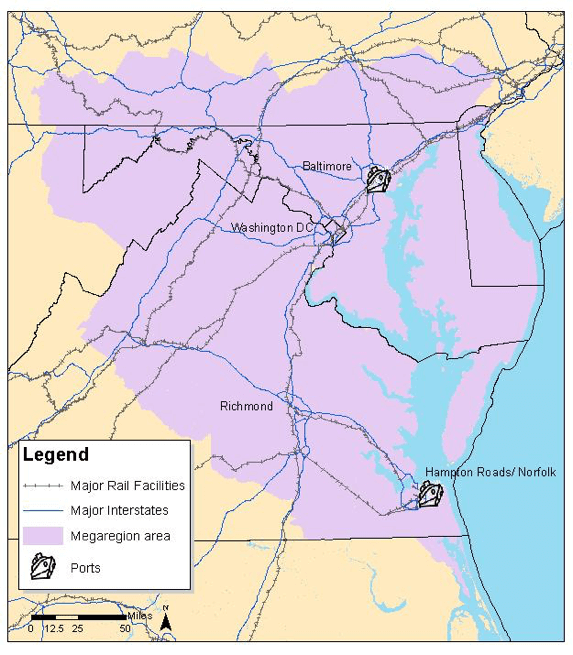
\includegraphics[scale=0.5]{graphics/48-chesapeake-bay-megaregion}
\caption{The Chesapeake Bay megaregion}
\label{fig:chesapeake-bay-megaregion}
\end{figure}

Given the geographic extent of a megaregion, a single scale model is insufficient to capture relevant activities, travel behavior, and their impacts. This fact is true for many statewide models as well, particularly if trips with external origins and destinations are modeled explicitly. Therefore, a two-layer approach was chosen to distinguish a megaregional layer represented in more detail and a national layer capturing relevant activities and flows outside of the main study area. Given the interactions between different megaregions nationally, and to some respect even globally, the two-layer approach facilitates to represent the study area with sufficient detail yet acknowledges that megaregions cannot be treated as monolithic islands.

\subsection{Model overview}\label{sec:cbm-model-overview}

The megaregion framework implemented for the CBM is shown in Figure \ref{fig:integrated-megaregion-model-concept}. A series of economic models predicts the growth and decline of different economic sectors based on assumptions of changes in the global economy. The economic models cover both the megaregional layer and the national layer to account for a global economy that affects growth and decline in the megaregion. The land-use model simulates changes in population and employment subject to this forecast.

\begin{figure}   % 49
\centering
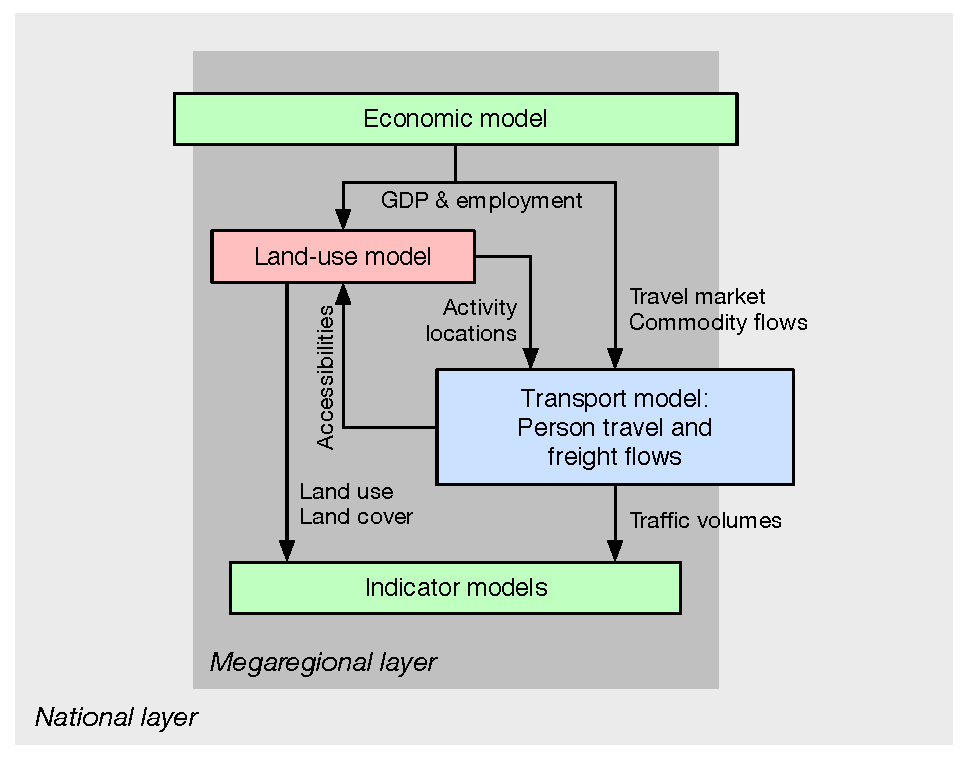
\includegraphics[scale=0.6]{graphics/49-integrated-megaregion-model-concept}
\caption{Concept of the CBM megaregion model}
\label{fig:integrated-megaregion-model-concept}
\end{figure}

The locations of population and employment are used in the travel demand model to simulate both person travel and freight flows. Accessibilities are fed back into the land-use model to influence land-use changes in the following simulation period, allowing land use to evolve over time. Finally, both traffic flows and the output of the land-use model are used in a series of indicator models to analyze the model results.

\subsubsection{Economic module}

To address the larger economic interest of a potential megaregion authority, the analysis framework emphasizes links with the economy, both nationally and locally. The megaregion model chain is driven by a national economic forecast component that predicts economic activity for large regions covering North America. The national Computable General Equilibrium (CGE) economic forecasting model built by the INFORUM group at the University of Maryland is applied \citep{mccarthy91}. The model employs inter-industry-macroeconomic general equilibrium models to examine past employment trends and to forecast future employment across 65 sectors of the economy. 

The primary model, LIFT (Long-term Inter-industry Forecasting Tool), uses econometric equations to predict final demand and output at the national level, based on inter-industry input-output relationships and value-added behavioral equations. The second component STEMS (State Employment Modeling System) allocates the national forecast to states, considering the industry's mix of basic and non-basic employment and personal income. Basic employment is driven by LIFT national industry trends, while non-basic employment is driven by state-specific personal income forecasts. The land use model further allocates these state control totals to model zones. Figure \ref{fig:county-level-flows} shows county level economic flows modeled for the CBM area.

\begin{figure} [!t]
\centering
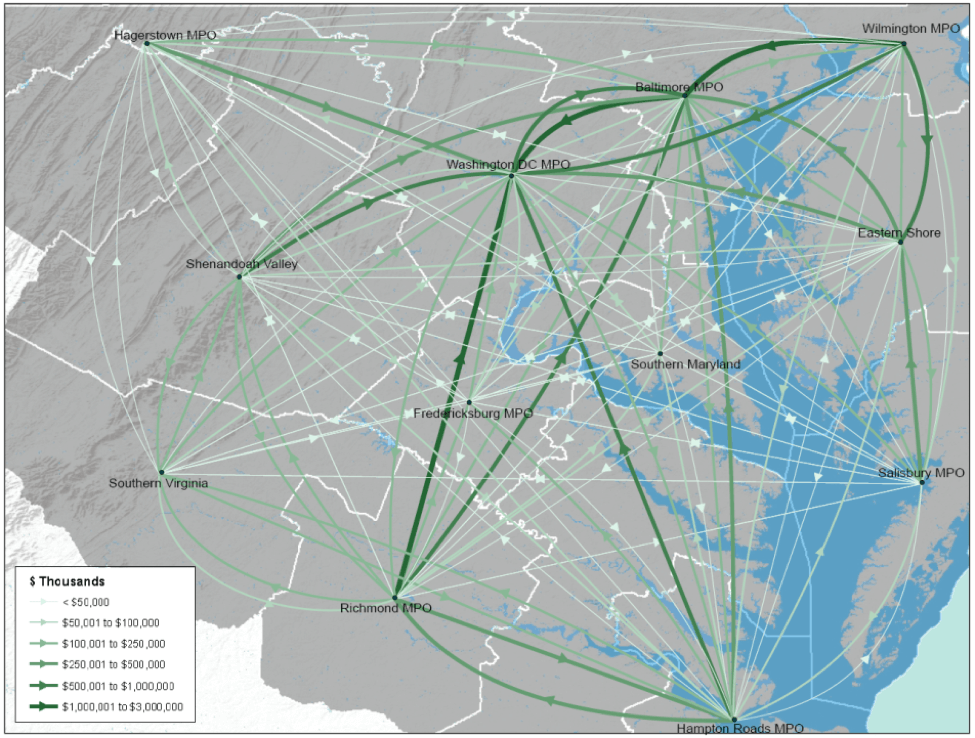
\includegraphics[width=6.5in]{graphics/50-county-level-flows}
\caption{County-level economic flows in the Chesapeake Megaregion}
\label{fig:county-level-flows}
\end{figure}

To account for local transport impacts on the regional economy beyond the national economic drivers that have little knowledge of local conditions, an economic post-processor was developed. The post-processor combines knowledge of county-to-county goods movement by industry and its sensitivity to travel impedance (generalized cost including time, distance, and travel cost per mile) to determine the impact of the local transport on each industry's supply chain relationships (up and downstream).

\subsubsection{Land use module}

The land use module works at two different geographies: a national geography with 126 zones covering North America and a megaregional geography with 2,075 zones. Economic flows generated by the economic model serve as control totals for the regional level:

\begin{itemize}
\item
  \emph{National Model:} Historic employment data from the U.S. Bureau of Labor Statistics Quarterly Census of Employment and Wages are disaggregated to counties. Employment data at the county level are used to calculate the share of employment in each county in the baseline years 2000, 2005 and 2009. The ratio of employment for each county is then extrapolated for five-year periods beginning in 2010 and ending in 2030 using an exponential smoothing method. Employment data from 101 BLS sub-sectors for the same period are then reconciled with 65 STEMS industries to match the BLS sub-sectors. This process simply employs a straight average of the two employment ratios. The purpose of this method is to allocate future STEMS projections based on the historic difference in BLS data and STEMS projections.
\item
\emph{Megaregional Model:} The local model generates socio-economic data at the resolution of megaregional modeling zones. The initial allocations are made based on transportation costs and the employment distribution of basic employment, or export-oriented employment. The allocation of households and employment is based on the Lowry model \citep{lowry64}.
\end{itemize}

The model is repeated in five-year increments until the horizon year 2030 is reached. The location of basic employment provides inertia in the allocation of non-basic employment. Obtaining data for a land use model at the scale of a megaregion is a challenging task, particularly if several states are involved. In contrast, a Lowry model requires less data but may provide reasonable land use sensitivities within computationally acceptable runtimes. Due to its simplicity and broad simplifications, the Lowry model has become rare at the urban level. At the megaregional level, however, such a model may provide the right balance between model sensitivities and comprehensiveness.

\subsubsection{Travel demand model}

Like the land use model, the travel demand model works at two geographic layers. While the local travel demand model is closer to a traditional statewide model, the national models are built from nationwide surveys for both personal and truck long-distance travel. Travel demand of the two layers is combined in the traffic assignment process that assigns short and long-distance traffic flows concurrently in a multi-class assignment.

The megaregional travel demand model is built as a five-step aggregate model that includes trip generation, destination choice, mode split, time-of-day split, and assignment. The original model concept was borrowed from the Baltimore Metropolitan Council model \citep{bmc07}, refined and applied for short-distance trips of 50 miles or less for the entire CBM study area. Trip generation rates were derived from a 2007 Household Travel Survey for the Baltimore and Washington D.C. metropolitan areas, as well as travel times, mode split and time-of-day split. Thereby, the model is calibrated to the core area of the CBM study area. A survey for the entire study area was not available.

This model includes a three-step local truck model based on the QRFM \citep{beagan07}, which was applied for local trips under 50 miles within the CBM study area. The comparison against VMT estimates revealed that the QRFM method, which is based on a 1992 truck trip survey from Phoenix, generated too many truck trips. Therefore, parameters were scaled down to resemble local VMT truck estimates and truck count data.

At the national layer, the National Estimate of Long-Distance Travel (NELDT) has been implemented to simulate long-distance person trips greater than 50 miles \citep{moeckel11}. The long-distance element of the 2002 National Household Travel Survey (NHTS), the most recent survey that covered explicitly long-distance trips in the U.S., provided data input. To expand the survey to cover all long-distance trips in the U.S., air travel data from the Bureau of Transportation Statistics (BTS), which covers 10 percent of all ticketed air travel passengers, was used as a control total to scale NHTS records to observed flight volumes. Auto trips were generated using the same scaling factor and added to the multi-class assignment with local traffic.

For freight long-distance travel, commodity flows from the Freight Analysis Framework FAF3 were used for truck trips of 50 miles or more. Though the 123 FAF zones reflect centers of economic activity, the resolution is too coarse to model truck trips on a network with much more detail. Therefore, flows between FAF regions were first disaggregated to flows between counties and then further disaggregated to flows between model zones. To disaggregate commodity flows, make/use coefficients and employment by type were used to allocate flows to the most likely producers and consumers of every commodity.

Commodity flows between zones are converted into trucks trips using average payload factors provided by FAF. These factors describe how many tons of a given commodity are carried by a truck on average. To account for empty truck trips, an empty-truck trips rate was added globally to all truck trips.

\subsubsection{Environmental and fiscal impacts}

A few indicator models were added to estimate the environmental and fiscal impacts. The results of the indicator models are not fed back to the other model components but were used to evaluate scenarios:
\begin{itemize}
\item
\emph{Gaseous Emissions:} This model captures traffic emissions using the EPA Motor Vehicle Emission Simulator (MOVES) model \cite{epamoves16}. The MOVES model uses VMT and link-level volumes and speed data output of the travel model to estimate GHG and other mobile emissions.
\item
\emph{Water Quality:} This model captures the impact of alternative policies on water quality. A nutrient-loading model estimated flows draining into the Chesapeake Bay. It forecasts the annual loads of nitrogen, phosphorus, and sediments. The model uses detailed land cover changes from a raster-based land use model to identify changes in nutrient runoff due to land cover changes.
\item
\emph{Infrastructure Costs:} This model estimates state and local governments' costs to provide public infrastructure in support of new development (e.g. roads, sewer, water). Established relationships between the current development and the provision of infrastructure were applied to project future improvements needed to satisfy additional settlement activity. Data included residential development classified by housing type, existing water and road infrastructure, property value trends and tax rates, among others.
\end{itemize}

\subsection{Lessons learned from the CBM model}

The design of the CBM model is similar to a statewide model. A comparable two-layer geography is represented in many statewide models to distinguish long-distance and short-distance travel. Special attention was given to add additional model components, such as economic, land use as well as environment and fiscal impact models, though many other statewide models use such ``add-ons'' as well. A significant challenge for the CBM was a study area that included parts of five different states and the District of Columbia.

While many statewide models cover parts of neighboring states at a higher resolution, it is rare that data from as many states are included. Creating a network from different sources, socio-economic data from different agencies and count data in different formats created a challenge for the development of the CBM. As such, the model was operational but only implemented as a prototype. Detailed model validation has never been conducted outside of Maryland.

As with many statewide models, the CBM coped with two levels of model integration (Figure \ref{fig:horizontal-vertical-integration}). On the one hand, vertical integration covers the interaction between different geographies, here the North America level with the megaregional level. On the other hand, horizontal integration captures the interaction between different modeling domains, such as transport models with land use models. A core finding was that the level of integration depends on (a) the frequency of information exchange, (b) the direction (one-way or bi-directional) and (c) software implementation constraints. Tighter integration turned out to not always be better. In some cases, lose coupling of models may be sufficient and much easier to implement.

\begin{figure}
\centering
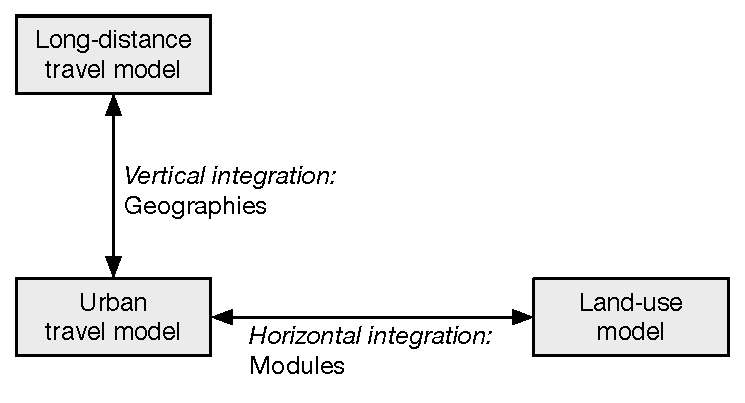
\includegraphics[scale=0.6]{graphics/51-horizontal-vertical-integration}
\caption{Horizontal and vertical integration in a megaregional model}
\label{fig:horizontal-vertical-integration}
\end{figure}

The work resulted in an extensive report \citep{ducca13} and a paper published \citep{moeckel15b}, but was never used as a true policy advice tool. Being funded by FHWA's Exploratory Advanced Research Program, it was not expected to be applied in practice. However, the work has not inspired the development of other megaregional models yet. Most likely, this is due to the lack of megaregional institutions across the U.S. that might use large-scale models to advise decision making. Therefore, the CBM model remains a proof of concept that may assist other megaregions in the future.

\section{Arkansas Statewide Model}

The Arkansas State Highway and Transportation Department (AHTD) completed a Phase II update of their statewide model in 2015. All parts of the model and underlying data were addressing during the update. The resulting modeling system represents an excellent example of best practices in statewide modeling, incorporating current thinking about how such models might evolve in the future. These qualities are shared by other models reviewed in this chapter. What makes Arkansas unique, however, is that they could leverage prior work and experience to do so within modest budget, and their creative approach to overcoming a lack of local travel behavior data.

A multi-scale modeling approach was employed to develop a model that provided a regional and national context for Arkansas, while still providing a high enough level of detail for accurate forecasting of policy and project scenarios within the state. The state is covered by 5,849 traffic analysis zones, designed to include urban model zones as already defined, and to be compatible with and nest within Census block and block group boundaries otherwise. Care was also taken to respect natural boundaries that impede flow, as well as not crossing major roadways and highways.

The rest of North America is covered by 144 zones formed by aggregations of Economic Areas defined by the Bureau of Economic Analysis (U.S. Department of Commerce) with the USA, and states and provinces within Mexico and Canada. Like many other statewide models, urban model networks within the state are fused with the FHWA National Highway Planning Network to represent the roadway system. A rail network maintained by Oak Ridge National Laboratory was used to represent the freight rail system.

Their model is described next, followed by a discussion of their innovative approach to data development and lessons they appear to have learned. Their model documentation, spread across eight reports, is available upon request from AHTD.

\subsection{Long-distance freight models}

Long-distance truck and rail flow forecasts are developed using four-step sequential modeling process, based upon commodity flow forecasts. Their model is based upon a 2008 Global Insight Transearch flow database. Unlike many states, who map the flows to truckload equivalents, the data are used to build a commodity flow model. This provides a degree of policy sensitivity that static forecasts, such as the Transearch and FAF static forecasts, do not. In this case changes in employment can be used as a proxy for changes in gross state product, growth in certain industries relative to others, and the like.

Linear regression models are used to predict annual tons shipped by all modes of transportation as a function of employment within industries that produce such goods, for 15 commodity groups. The production model was estimated at the county level within Arkansas, and state level outside of it, for 13 of those groups (reported flows in the Transearch data were used for mining and coal flows). The resulting r\textsuperscript{2} statistics ranged between 0.46 and 0.84, providing reasonable fits, Attraction models were likewise estimated using linear regression, using input-output tables to understand better the linkage between commodities and consumption. Special generators were developed for counties whose actual tonnage (from the Transearch data) deviated significantly from the regression estimates.

A doubly-constrained gravity model is used for trip distribution, using friction factors based on the distances coded in the Transearch data. The latter are often used instead of mathematical functions to replicate the multiple peaks in observed trip distance distributions. An incremental mode choice model, based upon existing mode shares by commodity and distance ranges, was developed using the Transearch data. The rail tonnage was assigned directly, with truck tonnage converted into daily truckload equivalents using payload and annualization factors. The latter were combined with auto flows in a multi-class traffic assignment.

\subsection{Person and other truck models}

Person local and external travel, as well as non-freight commercial vehicles, are modeled using the widely-accepted trip-based modeling paradigm, with a few interesting extensions. A schematic diagram of the modeling system is shown in Figure \ref{fig:arkansas-flowchart}. Nine person and four truck trip purposes are modeled, to include two of each devoted to external trips (i.e., those crossing the state border). Two of the purposes represent infrequent long-distance travel, which includes trips longer than 100 miles. Like an increasing number of states, person trip generation rates are differentiated by area types (four in this case, as a function of population and employment density) in addition to household size and income groups. Attraction rates were calculated using borrowed data, stratified by the same four area types and income groups, as well as total households and employment by broad categories. Special generator attractions were calculated for unique land use types, such as universities, hospitals, military bases, and airports.

\begin{figure}[!t]
\centering
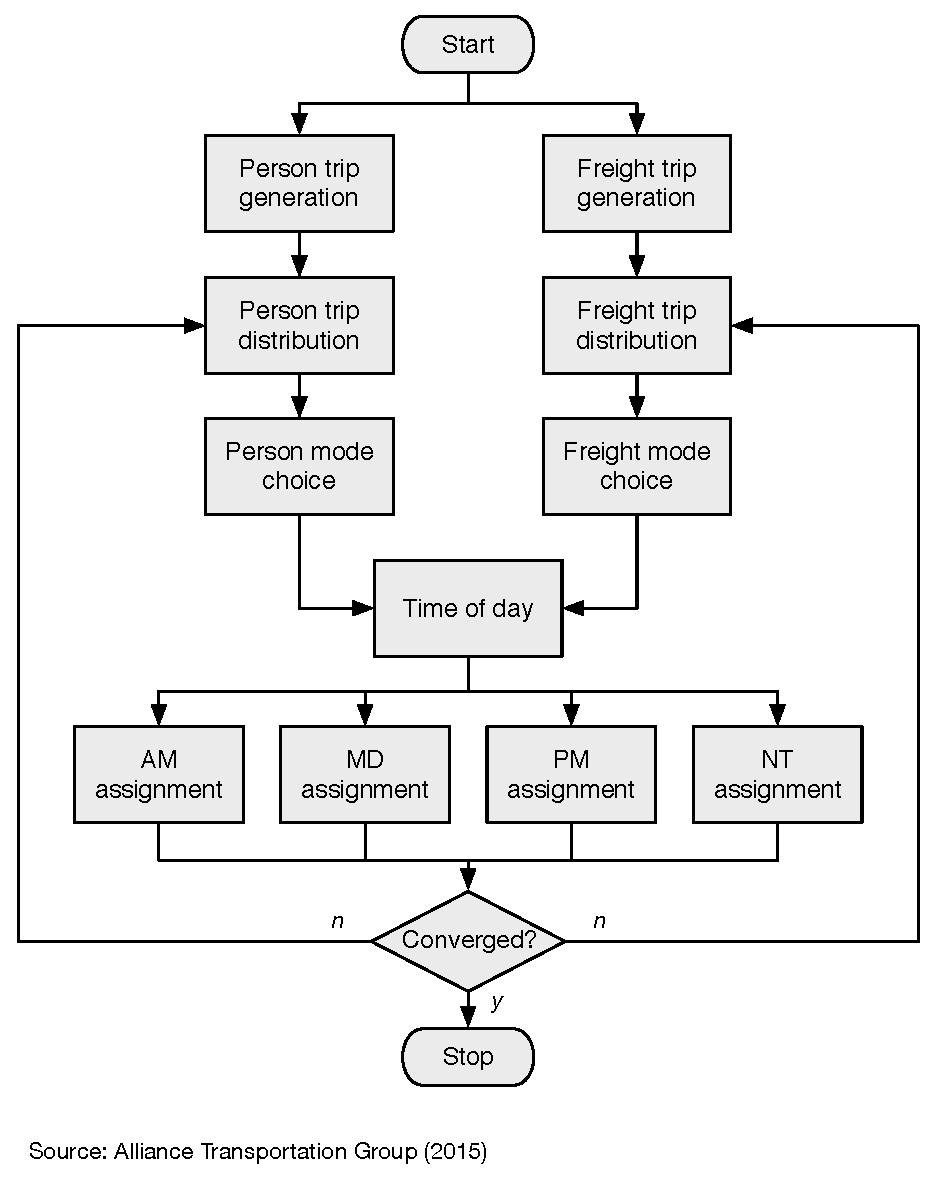
\includegraphics[scale=0.6]{graphics/52-arkansas-flowchart}
\caption[Schematic diagram of Arkansas statewide model]{Schematic diagram of Arkansas statewide model (Source: \cite{alliance15}}
\label{fig:arkansas-flowchart}
\end{figure}

Doubly-constrained gravity models are used for trip distribution, using distance as the measure of impedance for infrequent long distance trips, and travel time for all other trip purposes. Friction factors were fitted to smoothed trip length frequency distributions for each trip purpose, and iteratively calibrated to survey data. A nested logit mode choice model that handles both local and intercity travel was developed, based heavily upon Federal Transit Administration (FTA) guidance and typical practices. Several of the model coefficients were asserted, based upon FTA advice, and then calibrated to local conditions. Calibration targets were generated from 2009 NHTS data for auto trips, while data from two Arkansas transit agencies were used for transit trips. The daily person trips by mode were allocated to four periods of the day, using diurnal factors by trip purpose and direction. Finally, the person flows were converted into vehicle trips through the application of auto occupancy rates, where appropriate.

External trips are those with an origin, and possibly destination as well, outside of Arkansas. This corresponds to the familiar external-internal (EI) and external-external (EE, or through) trip purposes. Because both local and long-distance trips by Arkansas residents are modeled there is no need to include internal-external (IE) trips, for they are already accounted for within the modeling steps described above. Traffic and vehicle classification counts at the state border are used to constrain the flows to observed or forecasted levels. The external trips go through the same diurnal factoring as internal trips before being combined with them for traffic assignment.

The person travel models include truck flows that are not represented in the Transearch data described above. These include trucks making local trips, as well as non-freight trucks traveling over longer distances. They are modeled in a similar manner as persons, using data borrowed from Idaho. Regression models by truck type were developed for trip generation, which are assumed to also represent trip attractions. Trip distribution models like those developed for person trips were calibrated for three categories of trucks. Diurnal factors were borrowed from Idaho, and compared to those found in the literature and other statewide models. When combined with the long-distance truck trips described in the previous section these flows represent the entire population of trucks operating within Arkansas.

\subsection{Traffic assignment}

The Arkansas model includes both highway and freight rail assignment procedures. The former is carried out for four time periods and includes feedback loops to obtain more accurate travel times, as shown in Figure \ref{fig:arkansas-flowchart}. Several user classes are jointly assigned. Trip matrices are segmented by 18 combinations of trip purpose, auto occupancy, and income groups to define the user classes. This is more detail than thought to be used in most statewide models. A multi-class static user equilibrium assignment process is run separately for four periods of the day, with each converging through feedback separately.

The widely-used Bureau of Public Roads (BPR) volume-delay function is used to update link travel times during assignment. The model coefficients were updated in the Arkansas model, drawing upon experience in other states and the literature. Ten variants are used to capture differences in perceptions and values within each user class. The function coefficients are also segmented not only by functional class, but by whether the downstream node is a signal or stop sign controlled, or not an intersection. Considerable effort apparently went into derivation and testing of these coefficients, as well as sensitivity testing of toll costs.

A simpler assignment process was also developed, to be used to reduce the computational burden and data handling associated with a large number of user classes. Three user classes (passenger, commercial trucks, and heavy trucks) are used, although doing so precludes analyses of toll and high-occupancy lanes. The modeling system also includes the capability to assign freight rail tonnage or annual train equivalents on a simplified rail network. The origin-destination flows are assigned to the shortest distance path, rather than attempting to capture the complexity of rail routing decisions that include factors such as interlining cost, track ownership, and cost minimization. The goal is to visualize the spatial dimensions of rail traffic, not its exact routing, for which their method is quite adequate.

\subsection{Innovative data development}

The developers of the Arkansas model had to overcome several data shortcomings, with the lack of household and truck travel survey being the most significant. It is common in such cases to borrow or assert models, or synthesize them using data from different sources, and to calibrate the model to what local data are available. Like other states, the developers turned to the NHTS for this task. However, there are too few observations within Arkansas to build a statistically stable and reliable model from them. However, both Tennessee and Texas had purchased additional samples during the 2009 NHTS cycle, which proved invaluable for the development of the Arkansas model. Summaries from both states were compared during each step of the person travel model. The Texas data were used in each case, for their much larger sample size (22,255 households) was an order of magnitude larger than collected in Tennessee. However, the differences between them, as well as summaries of the small samples from other nearby states and 2003 household survey from Central Arkansas, defined the range of such values. This helped identify which patterns and relationships were the most stable, versus those where Arkansas would likely vary from its neighbors.

Similar data were borrowed for other parts of the model, to include:
\begin{itemize}
\item
Workplace surveys from Arkansas were similarly not available. The team obtained permission to use data from four Texas workplace surveys to develop trip attraction rates. The resulting rates compared well to other models and the literature.
\item
Typical mode choice model structures, parameters, and coefficients were drawn from FTA New Starts guidance, as well as advice from senior modelers in the agency. The collection of onboard travel survey data, coding and testing of transit networks, and formal estimation of parameter estimates is very time-consuming, and of questionable value in settings like these. Synthesizing these data saved the developers considerable time, permitting them to focus more time on calibration and sensitivity testing, both of which led to better modeling outcomes.
\item
Data from a 2008 commercial vehicle survey conducted for the Community Planning Association of Southwest Idaho (COMPASS), the MPO for the Boise area, were used to develop the truck characteristics in the person travel model (e.g., those trucks not included in the Transearch data, to include local and non-freight truck movements). These data proved invaluable for the development of that part of the model.
\item
Experiences with traffic assignment models, to include volume-delay function parameters, were heavily informed by models implemented in several other states by the developers.
\end{itemize}

The effective use of these data reduced both the cost and time required to develop the Arkansas model. Judging from the reported validation statistics, these borrowed data enabled the model to perform as accurately as reported in many other states. Thus, Arkansas has a fully functional model, when they might still be in development stages had they invested in a large-scale household survey across the state. In a sense, the availability of these data has made statewide modeling affordable for Arkansas, and therefore accessible when it might not otherwise have been.

\subsection{Lessons learned from Arkansas}

Arkansas is a relative newcomer to statewide modeling, having first embarked upon its first version in 2010, and recently updating it. They achieved this through leveraging work done elsewhere, as well as learning from their experience. Some of the more important and interesting successes include:

\begin{itemize}
\item
The NHTS is a very important resource for statewide modelers, for many states lack the resources required to conduct statewide travel surveys. However, little has been done to compare how estimates for one state stack up against its neighbors, or whether data from several states can be pooled in to gain acceptable sample sizes. Several developers have already done so, of course, but few compare the results in each step of the model like Arkansas has done. This underscores the importance of funding add-on surveys (i.e., paying for the collection of additional surveys) in future versions of the NHTS for those states unable to conduct such surveys on their own, as well suggesting the value of several adjacent states pooling funds to do so.
\item
Considerable work went into the development of a graphical user interface and standardized reporting, both of which make the system and its outputs more accessible to both modelers and their clients. Having a model that is easier to use enables AHTD staff to spend more time evaluating results, rather than setting up and running the model in an ad hoc manner.
\item
The focus was on the usability of the model throughout its development. This not only drove the initial design, but remained in focus when evaluating validation outcomes and deciding upon changes and possible model enhancements. This is best illustrated in their adoption of FTA guidance and advice in the construction of their mode choice model. Rather than developing a model and testing its utility, the developers started with a recommended approach and worked backward to determine how best to calibrate and test it. This approach saved considerable time and effort for a part of the modeling system that is often as costly as the rest combined.
\end{itemize}

Their current model appears capable of meeting their short-term needs, and represents a sound investment. How the model will evolve over time to address new and more complex issues not well addressed using trip-based modeling systems remains an open question. There is no doubt, however, that Arkansas is on a path that will enable them to do so in a highly cost-effective manner.

\section{California statewide models}\label{sec:ca-statewide-models}

On paper, California has the most expensive statewide model in existence, by a wide margin. While it is difficult to pinpoint the full cost of statewide modeling, the costs shown in Figure \ref{fig:resource-allocation} (page \pageref{fig:resource-allocation}) suggests that their costs far exceed those of other states. A closer look reveals that their program involves far more than just statewide travel modeling, and forward-thinking and ambitious investment in data collection that eclipses those of almost all other states. Moreover, there are two statewide models of California, which unto itself is an interesting story. Their modeling systems and what they can do with them, how they have partnered with others in their development, and how they might complement one another are described in this section.

Extensive and current documentation about both modeling systems is available online. These include descriptions of the models and their development, as well as reports about supporting data, results of model testing, forecasts developed using them. In the case of their HSR model the findings of an independent peer review panel are also published on the Authority's website. This might not seem remarkable today, until one attempts to find similar documentation for most other statewide models online. Viewed in that light, California is commendably progressive in making extensive documentation of their statewide travel data and models publicly accessible.

Each modeling system is described in the following sections, with a focus upon the unique and noteworthy aspects of each.

\subsection{The California Statewide Travel Demand Model}

The California Department of Transportation (Caltrans) has developed a comprehensive multimodal statewide model of all personal and commercial travel by residents of the state. The model system is used by Caltrans for a variety of analyses. The system was designed to meet several analytical needs:

\begin{itemize}
\item Provide insights into long-distance travel between and through multiple regions of the state
\item Model behavior for all California residents and firms, expressed as multimodal tours and trips
\item Provide data on external travel for urban and metropolitan travel forecasting models
\item Evaluate changes in greenhouse gas emissions, as required by several state laws
\item Provide aggregate travel statistics that can be used to resolve differences between adjacent urban and regional models
\item Provide a travel demand model for agencies that do not maintain a model of their own
\end{itemize}

Descriptions of the modeling system and data, as well as how they have partnered with other agencies, are presented in the next sections.

\subsubsection{Partnerships}

Caltrans has partnered with several agencies to fund and direct their statewide data and modeling program. The first-generation model was funded through university research, as is work on a new freight modeling framework. Their recent statewide travel survey, described below, was designed to collect data needed for both transportation and environmental models. The list of collaborators is impressive, and is unmatched by any other state except Oregon:

\begin{itemize}
\item California Air Resources Board
\item California Strategic Growth Council
\item California Department of Public Health
\item California Department of Housing and Community Development
\item California Energy Commission
\item California High-Speed Rail Authority
\item Metropolitan planning organizations
\item Regional transportation planning agencies
\end{itemize}

Not all partners are involved at the same level, but the statewide modeling program in California has greatly benefited, and had more resources at their disposal as a result. Granted, California has passed legislation requiring such collaboration to achieve sustainable planning and greenhouse gas reduction targets. Specific multi-agency mandates and deadlines are required in several laws, to include:

\begin{itemize}
\item California Global Warming Solutions Act (AB 32, passed in 2006)
\item Sustainable Communities and Climate Protection Act (SB 375, passed in 2008)
\item California Homes and Job Act (SB 391, passed in 2013)
\end{itemize}

Regardless of the motivations, the level of inter-agency cooperation and pooling of resources to solve large problems is helping to drive the agenda for statewide modeling, both directly and indirectly.

\subsubsection{Data development}

Many agencies rely on the NHTS or data borrowed from other areas to build their statewide models, as revealed in Table \ref{tab:data-combinations} (page \pageref{tab:data-combinations}). California, like a few other states, has opted instead to collect the data it feels are required for robust models. Some have no parallel in other places, and have enabled Caltrans to develop the advanced model that it currently uses. Two of the most important recent data collection activities
included:

\begin{itemize}
\item
The 2013-14 California Household Travel Survey (CHTS) collected data from households in all California counties, and three in Nevada \citep{nustats13}. A traditional 24-hour travel diary was used to record trips by all modes of transportation for all respondents, and in some cases, three types of GPS data collection (wearable, in-vehicle, and connected to the on-board diagnostics {[}OBD{]} port). Data were collected from the GPS units for periods of three or seven days, depending upon the device used. Households were also asked to also report long-distance travel over the past eight weeks using a separate retrospective survey. Complete data from a total of 42,431 households were collected, to include 5,717 from which GPS data were obtained. An additional dataset of partially completed surveys for 20,651 households was provided, which some of the survey sponsors considered still useful.
\item
The 2014 California Vehicle Inventory and Use Survey (Cal-VIUS) is designed to fill the gap left by the cancellation of the federal survey a decade ago. Like its national predecessor, they survey is designed to collect data on the physical and operational characteristics for a sample of all commercial vehicles. The survey, being conducted by the Institute of Transportation Studies at the University of California-Irvine, is being conducted in two parts. The first is a web-based survey of fleet managers, used to collect information about the vehicle and its annual operation. A driver survey is completed from a mobile phone app over a three-day period. These data will be invaluable for developing and validating the commercial vehicle models. The survey is currently in progress.
\end{itemize}

\subsubsection{Overview of the modeling system}

The second version of the California Statewide Travel Demand Model (CSTDM) was delivered in 2014 \citep{cambridge14-cstdm}. It is a multimodal, tour-based travel modeling system with five major components, as shown in Figure \ref{fig:cstdm2-structure}. All the models employ a microsimulation framework, in whole or in part. The SDCVM, for example, uses aggregate models to generate tours, and microsimulation to add their attributes. The system simulates travel by all California residents and firms, for a typical weekday in the fall or spring. Databases have been developed to support forecasts for 2015, 2020, 2035, 2040, and 2050. In a nutshell, the five components include:

\begin{figure}  % 53
\centering
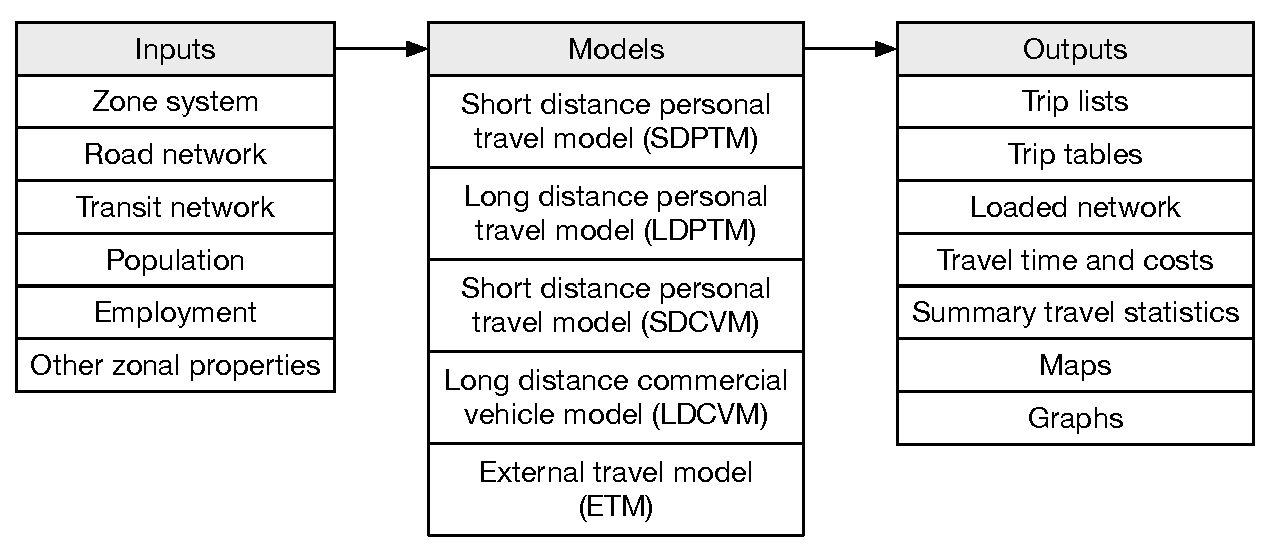
\includegraphics[scale=0.6]{graphics/53-cstdm2-structure}
\caption{Structure of the California statewide travel demand model}
\label{fig:cstdm2-structure}
\end{figure}

\begin{itemize}
\item
The SDPTM consists of a series of logit models that generates tours and trips by five periods of the day. Starting from a synthetic population, long-term choices are modeled first, to include work and school location and driver license status. Daily tours are then generated, as well as their primary destination and mode of travel. Secondary destinations are then chosen, followed by trip mode choice. The models are applied somewhat differently for each tour purpose.
\item
The LDPTM is based upon the approach used in the statewide HSR model, which begins with a tour formation model. It is run in parallel with the SDPTM. Tour attributes are then generated, with models of party formation (size), tour properties (duration and time of day), destination choice, and mode choice. The latter includes main, access, and egress choice models, based upon an earlier version of the HSR long-distance mode choice model. An interesting aspect is how both models interact, as shown in Figure \ref{fig:california-interactions}.
\item
  The SDCVM is an adaptation of a tour-based microsimulation of CV flows, based on a model originally developed in Calgary \citep{hunt07}, and based upon parameter values from its implementations in Alberta and establishment survey of California businesses. The model structure is illustrated in Figure \ref{fig:calgary-model}, which simulates flows from six categories of establishments, for three types of trucks.
\item
The LDCVM is based upon truck origin-destination flows derived from a PECAS model implemented in the first-generation statewide model. Growth factors are used factor the trip matrices for future years, based upon growth in zone-level demographics. While the original flows were developed using PECAS, the current model does not depend upon it for current or future forecasts.
\item
The ETM models handle flows to and from 51 external stations in the model, including three marine ports. They are organized into six districts across the state. Existing counts at the external stations, and extrapolations into the future, are used to generate external trips. A logit-based destination choice model is used, and trips are allocated to time periods using observed patterns.
\end{itemize}

\begin{figure}  % 54
\centering
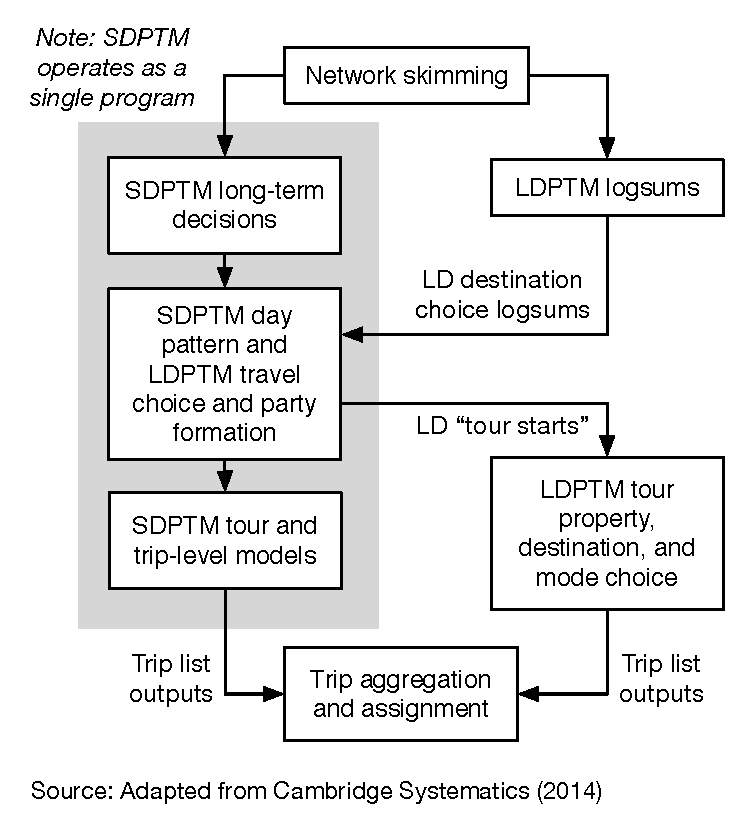
\includegraphics[scale=0.6]{graphics/54-sdptm-ldptm-integration}
\caption{Integration of the California short and long-distance person travel models}
\label{fig:california-interactions}
\end{figure}

\begin{figure}   % 55
\centering
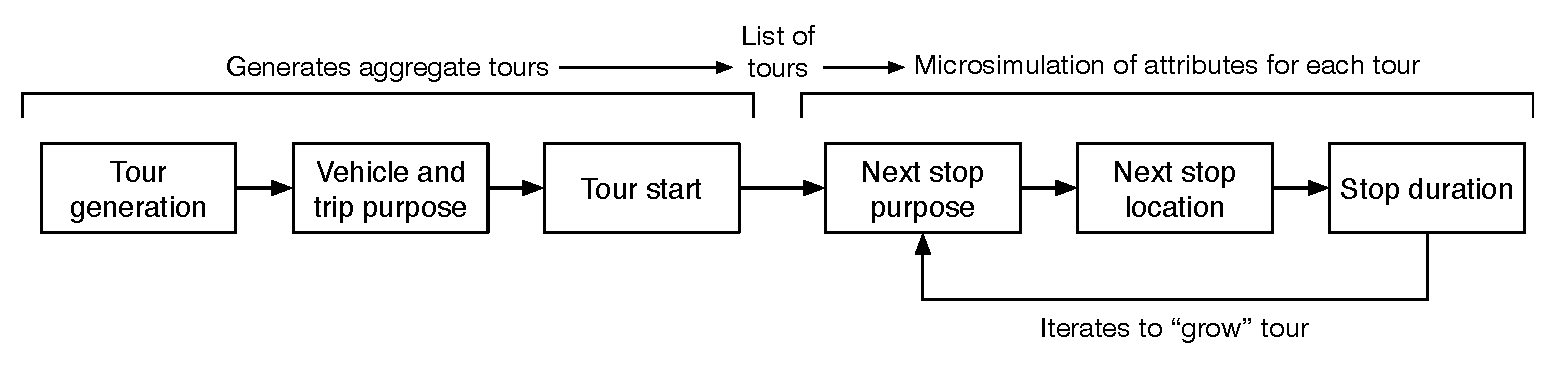
\includegraphics[width=6in]{graphics/55-calgary-model}
\caption{Structure of the Calgary commercial vehicle model}
\label{fig:calgary-model}
\end{figure}

The resulting modeling system includes 5,474 traffic analysis zones, which nest within California counties and 524 land use zones used by the PECAS model \citep{hunt05}. The latter was an integral part of the first-generation statewide model, but is not an active part of the current version. The network includes over 325,000 nodes, including its sparse representation of the national Interstate and US highway system.

One innovative feature is the use of a simplified representation of local transit service, using a technique described by \cite{circella14}. Fixed guideway and intercity transit lines are explicitly represented in the model, but the level of service times and costs are synthesized based upon roadway speeds, land use variables, and assumptions about transit service levels. The same methodology is used in the Oregon statewide model, to obtain reasonable approximations of local transit accessibility without the huge effort required to code every local bus line within the state.

\subsubsection{Next steps}

Caltrans plans to complete model updates on a five-year basis, incorporating data that has become available or been updated since the last update. Caltrans is sponsoring the development of a new multimodal freight model that will eventually replace the long and short-distance commercial vehicle models in the current system. Both steering committees and peer review panels will be used to provide advice about the long-term evolution of the statewide model and its supporting data programs.

\subsection{The California High-Speed Rail Ridership and Revenue Model}\label{sec:california-hsr-model}

The California High-Speed Rail Authority maintains a separate ridership forecasting model, used to support business and system planning, as well as corridor studies and analysis of alternative alignments and phasing of implementation. It is a complete statewide model, and uses some of the same data used to develop the Caltrans model. It incorporates a more sophisticated mode choice model better suited for evaluating HSR alternatives, but otherwise covers the same travel markets as the Caltrans model, and at comparable levels of spatial, temporal, and behavioral resolution. It also includes an explicit risk and uncertainty assessment process. This is a necessity for HSR forecasting, but unfortunately unique among the statewide models reviewed for this report.

The Authority oversees the ridership forecasting work, with assistance from their Rail Delivery Partner (RDP) and an independent peer review panel. However, all model development and application work has been undertaken by Cambridge Systematics, under contract to the RDP. The associated cost of developing and using this model is not published, but is thought to be comparable to the investment made in the Caltrans model and data. Moreover, scores of forecasts have been produced with it. Because these were undertaken by the consultant those costs likely account for a significant portion of the total cost incurred by the Authority.

Several aspects of the California HSR model and how it is used are noteworthy. A summary of their modeling system, as well as data and institutional aspects of its development and deployment, are described in the following sections.

\subsubsection{Open and transparent analytics}

The California HSR model is unique in several aspects, both in comparison to other HSR forecasting efforts and most other statewide models. Most HSR forecasts, both domestically and abroad, have been undertaken by consultants that use proprietary models and data to develop them. The overall approach is described in their reports, as well as characterization of major market trends driving the trajectory of the model. Narrative, tabular, and graphical summaries of the forecasts are also provided, along with their interpretation. However, the forecasts are the delivered product, not the data or models used to develop them. This precludes reuse of the data and models, as well as detailed review and testing. California breaks from that tradition, having developed the data and platform used for their analyses. This gives them the ability to test new alternatives quickly, as well as generating new forecasts to reflect changing alignment, service levels, fares, etc. It should be transferable to other regions, although no known attempt has been made to do so.

The model was originally developed under contract to the Metropolitan Transportation Commission in the Bay Area. It was based, in part, upon results from stated preference surveys carried out in 2005 within the state and older statewide travel survey data. It was subsequently extended to support statewide analyses for the Authority, and updated with new data and models. The current version of the system, known as the Business Plan Model-V3 (BPM-V3) incorporated new survey data from the CHTS and a 2013-14 SP survey performed for the Authority, a completely revised mode choice model, and improvements to almost all the other modules.

The model is extensively documented \citep{cambridge16-bpmv3}, as are the data used to develop and apply it. Documentation about the model structure, key parameter values and their derivation, and tests of the effect of major assumptions are available on the Authority's website.

\subsubsection{Data development}

An intercept survey of stated and revealed intercity mode preferences of California residents was undertaken in 2013-14. Data about respondent attitudes towards, and experience with, HSR elsewhere were also collected. The data, and how they compared to results obtained in an earlier survey completed in 2005, were used to develop a new mode choice model \citep{cambridge15-hsrts}. The stated preference (SP) portion consisted of six experiments presented to each respondent, consisting of several options for mode of transport and variations on important characteristics of each. A total of 4,314 respondents provided complete and usable data. About 40 percent were from conventional rail riders, while the remainder were split almost evenly between air and auto travelers.

The results of the CHTS, and particularly the long-distance element, were also used in model estimation and calibration. The daily diary portion of the survey was large enough to accurately portray the incidence of long-distance travel on the survey day, something smaller surveys struggle to capture. While the number of such observations was too small to build robust models, the CHTS travel diaries did prove useful for validating the incidence of long-distance travel. Information about the latter was also gleaned from an additional eight-week recall survey of long-distance travel. This optional part of the CHTS provided data on 32,641 long-distance trips by California residents, which was used for some parts of model development, and validation of other parts. The aggregate results were also adjusted based on 2011 data from a Harris Panel survey, to understand gaps in the data, particularly with respect to uncertainty about how CHTS respondents reported repetitive trips.

\subsubsection{Bi-level modeling framework}

The modeling system employs the bi-level structure shown in Figure \ref{fig:bpm-v3}. The long-distance model includes trips within the state longer than 50 miles, stratified by four trip purposes. They include business, commuting, recreational, and all other trips, a common scheme used in long-distance travel models. The trip frequency and destination choice models were estimated using the CHTS long-distance survey data and revealed preference (RP) portion of the 2005 RP/SP survey. The mode choice model is a combined model of main, access, and egress mode choice, estimated from the weighted RP/SP surveys alone. Several nesting structures were tested, and the final model was calibrated using the expanded CHTS, rail boardings, and air travel flow data.

\begin{figure}   % 56
\centering
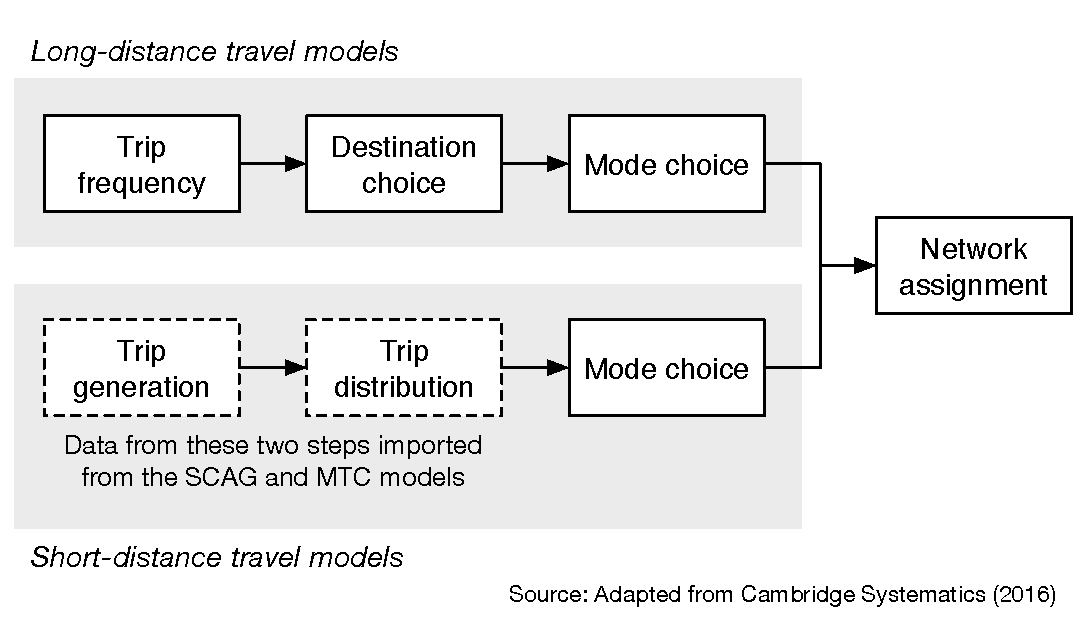
\includegraphics[scale=0.575]{graphics/56-bpm-v3}
\caption{Structure of the California HSR Business Plan Model-V3}
\label{fig:bpm-v3}
\end{figure}

The short distance model includes person trip tables by mode and trip purpose from the regional travel models used by the Southern California Association of Governments (SCAG) and the Metropolitan Transportation Commission (MTC). They are the metropolitan planning organizations for the Los Angeles Basin and San Francisco Bay Areas, respectively. Trip tables for their base and forecast years are used to represent short-distance travel within the BPM-V3 framework, and are translated into the format required by the short distance mode choice model.

The mode choice model is an adaptation of the 1996 Baycast model developed for MTC, which has been calibrated to reproduce base year transit ridership within each metropolitan area. More recent models in both regions are further apart in structure, precluding their direct use within the BPM-V3 framework. The resulting system provides consistent forecasts of short-distance mode choice within both regions. The station spacing outside of those regions is too far apart to enable short-distance HSR trips, obviating the need for short-distance models within the rest of the state.

The BPM-V3 system and its predecessors have been used to generate ridership and revenue estimates for initial and detailed system planning and in support of corridor studies and evaluation of candidate initial operating segments. This has included the environmental studies required at all levels of analyses for the program, and use for station-level impact analyses. The latter has required post-processing of the model outputs, for the model was not designed to support detailed analyses at a fine level of geography. The SCAG and MTC models are well-suited for that level of analyses, but only for station-level analyses within their modeled area. 

The BPM-V3 and its predecessors have also been used to generate forecasts for the Authority's biennial business plan. The process used to develop the forecasts and their interpretation is described by \cite{cambridge16b}.

\subsubsection{Independent peer review}

The early forecasts developed using the first version of the model were heavily criticized with respect to their derivation and accuracy \citep{brownstone10}. The Authority formed an independent peer review panel of prominent experts in travel demand forecasting to review the entire modeling system, not just those parts at controversy, and advise the Authority on its fitness for use. The Panel conducted a thorough review over a period of several months, and made several recommendations that guided the development of the second and third versions of the modeling system.

The group was renamed the Ridership Technical Advisory Committee in 2014, as their role changed from the independent review of the original model to providing advice to the Authority on long-term goals for their forecasting work, review of interim products, and continued review of technical aspects of the modeling system. Their work and findings are reported in over a dozen reports published on the Authority's website.

\subsection{Lessons learned from California}

Several regulatory and policy issues seemingly unique to California have influenced how their statewide models have evolved. However, climate change, economic interaction, sustainability, and new technologies are issues that other states are beginning to grapple with as well. Some of the key lessons learned from California include:

\begin{itemize}
\item
The importance of, and value gained from, data collection cannot be overstated. California has invested heavily in person and freight travel data collection, and is committed to continuing these programs in the future. This has enabled them to gather information about their unique local markets, overcome long-standing gaps in knowledge about intercity modeling, learn how California residents might react to new modes of travel and changes in existing ones, and focus the survey upon information required for their advanced models.
\item
Caltrans was not afraid to significantly overhaul the statewide model, enabling them to refocus their efforts on aspects that proved important during use of their first model, and streamline other parts of it. Doing so was costly, but provided them with improved model performance and capabilities.
\item
Their investment in rigorous peer review enabled the High-Speed Rail Authority to quickly address controversy about the model and forecasts generated using it. Such a group not only brings new ideas to the table and asks hard questions, but they also bolster the credibility of the agency. This is important in cases where new modeling approaches are being used, or when major decisions are being made based on the forecasts.
\item
There is more similar than unique about both California models, enabling them to share data and lessons learned. The ability to compare one to the other, especially in model calibration and validation, is particularly valuable.
\end{itemize}

Very few states have had the courage or resolve to reinvent their statewide modeling programs in the way that California has. Their commitment to data collection is especially laudable, for it has enabled them to break past the barrier of knowing little about patterns unique to California, and their interactions with external markets. These progressive ideas will hopefully define a new standard in statewide modeling in North America.

\section{Florida Statewide Model}

The Florida Statewide Model is a particularly interesting case study for this report for two reasons. First, the consistency between MPO models and the statewide model in terms of input data and model design is remarkable. Secondly, the Florida DOT staff appears to be doing an excellent job in explaining the value and limitations of statewide modelling to decision-makers and other. This might be part of the reason why, per the survey, Florida has retained the largest number of staff members working on statewide modeling among all state DOTs in the US (even though Florida is only the fourth biggest state by population). The combination of continuous exchange with potential model users and a strong champion promoting statewide modeling appears to have established the statewide model as an integral part of transportation planning in Florida.

Florida's statewide modeling efforts started in 1988 with software written in Fortran and TRANPLAN, making Florida not the first but one of the early adopters in statewide modeling. Like other states, Florida's intention was to model travel demand outside and between MPO areas, where much of Florida's population growth has been occurring over the past two decades. Highway corridors are of particular interest, as well as long-distance freight flows. In 2000, the model was transferred to Citilabs' CUBE transportation modeling package.

\subsection{Coordination between statewide and MPO models}

In Florida, statewide modeling and MPO modeling are closely coordinated. The Florida Standard Urban Transportation Model Structure (FSUTMS) has been developed to serve both statewide and urban modeling needs. The FSUTMS provides the same model structure for statewide and urban models, including model scripts, software, zone systems, networks, socio-demographic data, and concepts for model application. These standards were developed by a so-called Modeling Task Force (MTF), consisting of representatives from MPOs, Florida DOT districts, Florida's Turnpike Enterprise, transit agencies, users' groups and FHWA. In addition, five technical committees were formed under the MTF: Data, Freight, GIS, Model Advancement and Transit Committees. 

These committees meet regularly in person or via web and serve as the technical backbone of MTF's modeling standards. These committees make recommendations on data purchases, model development and model applications. Other transportation professionals throughout the state, including academics and consultants, participate in discussions and technical committee activities without voting rights. The Florida DOT maintains a website for all model users in the state to provide updates on model development, data, and joint activities \citep{floridadot16}. Finally, FSUTMS also provides training workshops free of charge to transportation modelers. Training topics covered in the past include CUBE scripting, express lane modeling, data for calibration and validation, destination choice, and others.

The consistent model and data structures for statewide and urban models allow close cooperation between agencies involved in transportation modeling in Florida. Data are stored in a hierarchical system where the statewide model serves as a data resource for all MPO models. A model update implemented in the statewide model can easily be transferred to MPO models, and vice versa. This close integration provides consistency across models in Florida rarely seen elsewhere. Expenditures for model development and data can be shared among agencies, making investments more efficient than in agencies that work in parallel.

On the flip side, the statewide transportation model needs to carry considerable detail that is relevant for MPO models. For example, the statewide model includes all urban model TAZ, adding up to 8,518 zones for Florida. With an additional 594 zones in Georgia and Alabama and 185 zones for the rest of the world, the Florida statewide model is one of the most detailed models in the country in terms of spatial resolution. Despite the detailed spatial representation, the statewide model can complete a model run overnight, including person and freight travel. Florida DOT carefully reviews model improvements on runtime and attempts to balance increased runtimes with added value.

\subsection{Model structure}

The person transportation model is a rather traditional trip-based, 3-step travel demand model. Florida's Turnpike Enterprise has developed a separate model that validated very well and has been used to provide input data for the development of the statewide model. Travel demand from the turnpike model and traffic counts were used in a Synthetic Matrix Estimation (SME), sometimes called Origin-Destination Matrix Estimation (ODME), to provide county-specific trip generation rates. While those rates were somewhat artificially created based on traffic count data, this approach allowed distinguishing significant differences in travel behavior between coastal and inland regions. Special generators for airports, ports and Walt Disney World have been added to trip generation. Trip purposes include home-based work, home-based shop, home-based recreational or social, home-based other, non-home-based, external/internal and truck/taxi. Truck/taxi accounts for short-distance trips (\textless{} 50 miles) of commercial vehicles and is based on a QRFM approach (compare \S\ref{sec:cbm-model-overview}).

Trip distribution follows a traditional gravity model approach, taking into account travel times and tolls. It has been k-factored using the above-mentioned turnpike model as well as NHTS data. Trip distribution was adjusted at the zonal level to closely match observed travel. Mode choice is limited to an auto occupancy model at this point. The trip generation rates used in the statewide model only cover auto trips, making mode choice superfluous. When trip rates are transferred to MPO models that include transit, they need to be increased accordingly. Florida DOT is currently working on a statewide mode choice model that is expected to include the modes auto (by occupancy), bus, rail and air.

External trips are generated at 59 external stations along the state border with Georgia and Alabama. These include internal-to-external (I-E) and external-to-internal (E-I) trips. External-to-external (E-E) trips were considered, though given the peninsular topology of Florida, E-E trips barely exist and have been excluded. External trips are split into ``local'' external trips of less than 50 miles and ``long-distance'' external trips that are between 50 to 200 miles. Short and long-distance external trips are calibrated separately using different gravity models.

The freight model called FreightSim is the newest addition to the Florida Statewide Model, completed in spring 2016. While the person travel demand model was implemented by AECOM, the freight model was added by RSG. This model was originally developed for Chicago \citep{outwater13} with FHWA funding and then transferred to Florida. The model starts with synthesizing firms by 20 industry categories and seven size categories for the entire U.S. Based on input-output tables, commodities by 43 SCTG categories are produced and consumed by each synthetic firm depending on their industry category. Next, supplier firms are selected, i.e. producers of a given commodity are linked with consumers of that commodity. The supply chain of goods flows may travel through distribution centers and warehouses; such alternative ``paths'' are evaluated, and the preferred path is chosen with a multinomial logit model. Shipment size and shipping frequency are selected next using a discrete choice model. Finally, a mode choice model using a multinomial logit formulation is used to select modes and mode combinations, including road, rail, air and waterway.

The criteria for selecting a mode include travel time, costs, characteristics of the shipment (e.g., perishable, expedited, containerized), characteristics of the distribution channel (i.e. whether a shipment is routed through a warehouse or distribution center) and whether the shipment includes an intermodal transfer (such as truck to rail to truck). On the truck side, the model further distinguishes heavy and medium trucks. 

In contrast to the person travel demand model, the freight model is cutting edge and one of the most advanced statewide freight models applied in the country. Florida DOT makes a concerted effort to balance the level of innovation with benefits for the task at hand. According to respondents from the Florida DOT, consultants sometimes try to push for more complex models, while the DOT attempts to carefully assess the ``return of investment.'' They also reported that in some cases simpler models fulfill their needs. The fact that Florida DOT decided to move their freight model to one of the most complicated models on the market underlines the relevance of freight in their statewide transportation planning. At this point, there are no plans to upgrade the person travel demand model by the same degree.

The network covers the entire country, with more detail in Florida and a decreasing degree of detail outside of Florida. Network resolution and zone system resolution decrease in detail similarly and gradually the further one travels away from Florida.

The Florida Statewide Model does not distinguish time-of-day periods but generates daily traffic. The assignment algorithm is a static user equilibrium approach. Traffic counts were available on 14,726 links (eight percent of all links in the network). After careful review of count data and elimination of implausible counts (such as counts that changed substantially from one year to the next), the model validated remarkably well. With a Root Mean Square Error between counts and modeled volumes of 44.4 percent and a correlation of R\textsuperscript{2} = 0.81, the model validates better than most other statewide models. In part, this may be due to the k-factoring of trip generation and trip distribution, and the simplification of not having to model mode choice.

\subsection{Model applications}

The Florida Statewide Model was designed with rather common scenarios in mind. Model applications focus on statewide analyses of traffic flows, corridor analyses and analyses of areas outside of MPO model study areas. Typical scenarios tested with the Florida statewide transportation model include:

\begin{itemize}
\item Operation analyses
\item Level-of-service analyses across the state
\item Performance measures for future years
\item Roadway projects
\item Support of the statewide Long-Range Transportation Plan (LRTP)
\item Freight analyses, particularly in relationship to port activities
\item Evaluation of reversible-lane counter flows versus allowing hard-shoulder flows
\item Corridor analyses
\end{itemize}

Current top priority is the analysis of reversible lanes and hard-shoulder flows. Freight is expected to play a much larger role in the near future, though given that the advanced freight model was completed only recently, possible applications have not been defined yet.

One common application the statewide model is not prepared to handle in its current state relates to managed lanes with variable tolls  throughout the day. As the statewide model covers daily volumes only, time-of-day dependent tolls cannot be modeled. At this point, such scenarios are handled by the turnpike model that has a finer temporal resolution. The Florida DOT is currently exploring the possibility of using a DTA model for selected corridors to model managed lanes with travel demand data from the statewide model.

\subsection{Future development}

The present base year is 2010 and the future year is set to 2040. Florida DOT is currently updating these years to 2015 and 2045. There are plans to replace the current stick network by a HERE network to provide enhanced spatial resolution and improved visualization of traffic patterns. Florida DOT is considering a destination choice model that would replace the gravity model in trip distribution as well as a mode choice model that would add travelers by bus, rail, and air.

Particular attention is given to tourist travel. At this point, external travel is represented rather simply through count volumes at external stations and special generators at airports. In the future, Florida DOT envisions generating synthetic travelers that visit Florida and follow selected activities. Like the activity-based modeling concept, tourists shall be modeled in much more detail to reflect their relevance for the state revenues. The tourist model shall be sensitive to, among other factors, increases in energy prices.

To further improve freight modeling, a tour-based truck model is envisioned as well. The FreightSim model system was originally developed with a tour-based truck model for Chicago. In Florida, however, it was decided to implement the freight demand generation first, gain experience with the model system and consider tour-based truck assignment at a later point.

Special effort is given to vehicle flow data collection. Being frustrated with the level of detail provided by commercial vendors of passively collected data, the Florida DOT has started collecting their own data in-house. Over 1,000 Bluetooth sensors are used across the state to monitor vehicle flows. Volumes and speed can be gathered from these data collection points. A few portable Bluetooth sensors can be located near gates that are predominately used by trucks, such as driveways near ports. Sensing the same vehicles at other screenlines throughout the state allows Florida DOT to understand truck flows specifically.

Over the last ten years, Florida DOT has invested about \$1 million per year into their statewide model. This includes expenditures for data and consultant fees but excludes salaries for DOT staff. While this is roughly twice as much as spent by the average state DOT in the US, the expenditure appears rather moderate given the size of Florida and the extra effort the DOT provides through supporting modeling for all MPOs in the state.

\subsection{Lessons learned from Florida}

The Florida DOT makes a concerted effort to explain the benefit of statewide modeling to model users and decision makers. Their survey respondents stated that they are at risk of being in constant ``model-update mode,'' overlooking valuable applications using the existing model. The Florida DOT attempts to be highly responsive to model requests; in cases where the model is not suited to fulfill the request, staff at the Florida DOT attempts to provide other data that may help answer the question, even if the originally requested information cannot be provided by the statewide model. At the same time, the modeling team at the Florida DOT attempts to market their efforts proactively to decision makers and staff members in other agencies. Explaining the relevance of statewide modeling helps to keep the program alive and relevant. Specifically, the Florida statewide model is actively used to provide input to:

\begin{itemize}
\item The state's highway maintenance program,
\item The Long-Range Transportation Plan (LRTP),
\item MPO transportation modeling efforts, and
\item The development of port models.
\end{itemize}

In addition, the agency keeps staff that is working exclusively on training in model applications. To fit into tight schedules of busy employees, the team developed 15-minute training sessions that cover selected topics, such as model convergence, managed lanes or external travel.

The Model Task Force described in the introduction to this case study turned out to be an excellent vehicle for bringing everybody on the same page regarding transportation modeling. Regular meetings ensure that people are informed and have a forum to contribute to model development and application. Annual technical meetings and annual application conferences have been instrumental in bringing together experts and advertise the potential of transportation modeling. These meetings have also helped to some degree to reign in unreasonable expectations of what models would be able to accomplish.

The biggest challenge for the Florida DOT remains the turnover of staff. Too many times has the agency invested into new employees who, once they were well-trained, decided to move into industry. This ongoing shift in personnel requires continuous training of new hires and consumes a substantial amount of resources.

\section{Oregon Statewide Model}

The Oregon statewide model has been under development since 1998, under the auspices of Oregon's Transportation and Land Use Modeling Improvement Program (TLUMIP). The modeling system seeks to fully integrate economic, land use, and multimodal transportation models within a single framework, with linkages to various evaluation and impact models. It motivated a revival in land use-transportation modeling in the USA, and spawned the development of models used elsewhere. The second generation statewide integrated model (SWIM2) is likely the most ambitious statewide model currently in operation in North America, and the first land use-transport model operated at the statewide level.

\subsection{The Oregon modeling context}

Oregon has pushed the envelope in land use planning over the past two decades, particularly in the Portland region. An effort was made at the outset of TLUMIP to identify the likely constituents of the model and the issues they were facing. These includes legislative staff, decision-makers within the Oregon DOT, and metropolitan planning organizations. At that time the interactions between land use and transportation were of high priority, and heavily influenced the design of the modeling system.

A little over a decade later the policy focus had shifted considerably. Applications of the first-generation model focused more on the interactions between the economy, jobs, and transportation than land use. Strategies for reducing greenhouse gas emissions had become an important topic, as did pricing, least cost planning (then a priority within the Department), and effects of the 2008-10 economic downturn.

At this writing, most of the previous issues remain, but several new ones have arisen. The ability to understand dynamic pricing remains a priority. Perhaps even more pressing is the need for information about the likely effects of connected and automated vehicles, which appear closer to reality than just a few years ago. Related to that are mobility services such as Uber and Lyft, and many others like to enter this space. These will change auto ownership patterns, as well as car and ride-sharing possibilities. Taken together, these requirements point to the need for a highly flexible and scalable modeling framework that can quickly adapt to new needs. Oregon has invested in strategic visioning models (\S\ref{sec:strategic-visioning-models}) and agile development (\S\ref{sec:oregon-statewide-integrated-model}) to help meet these needs, and they continue to seek new approaches that will enable them to do so.

\subsection{Data development}

The first phase of TLUMIP demonstrated the proof of concept, proving that large-scale land use-transport modeling was feasible and capable of meeting agency needs. A statewide model was implemented within the TRANUS framework \citep{delabarra05}, and the initial development of an urban model in Eugene-Springfield evolved into the initial version of UrbanSim \citep{waddell02}. A considerable amount of effort was devoted to assembling the data required to build both models. The goal in both cases was to create the initial models using secondary data sources, both to reduce their cost and implement them quickly. Oregon did not have a prior statewide model, necessitating the development of zone systems and networks from scratch, as well as data unique to land use-transport models. The latter included land pricing data, parcel, and tract level databases, and economic input-output flows and coefficients. Surveys were conducted at truck weigh stations to better understand the relationship between tonnage by commodity and truckload equivalents.

The required socio-economic and land use data are unusually detailed for a statewide model. They include:
\begin{itemize}
\item 18 household types, stratified by household size and income
\item 52 employment categories
\item 14 occupation categories
\item 6 residential floorspace types
\item 14 non-residential floorspace types
\item 41 SCTG commodity classifications
\end{itemize}

A statewide household travel survey of 14,000 households was carried out in 1998-99. It was designed to support the development of small urban and MPO travel forecasting models, as well as the statewide travel models. The Oregon Household Activity Survey (OHAS) of around 18,000 households was subsequently conducted in 2009-11. Both surveys included households across the state, with about 6,500 of them within the Portland-Vancouver metropolitan area as part of the OHAS. Oregon has otherwise relied upon secondary public or government data sources, or have purchased third-party data, to support their modeling needs. Like other states, they have borrowed data from other places, to include long-distance travel survey data from Ohio's 2001-03 statewide household travel survey. Like many other states, Oregon uses the FAF data to depict commodity flows entering or leaving the state. These data are fused with Carload Waybill Sample data to better understand rail traffic patterns.

\subsection{Statewide Integrated Model (SWIM)}\label{sec:oregon-statewide-integrated-model}

Work began a decade ago on the current statewide model, after completing several applications with the first-generation prototypes. It was decided to focus on a single framework, rather than separate models at the urban and statewide scales. A modular approach was adopted, where each component would interact with others through data files and messaging. This was thought to facilitate the development of each module by different teams, as well as testing different approaches for each, without disrupting the work of others. The resulting modeling platform is a hybrid, in that some models are aggregate equilibrium models, while others are microsimulated. The modeled area covers the state of Oregon and a halo of roughly 50 miles covering counties in the neighboring states of Washington, Idaho, Nevada and California. A multi-scale system is used to represent geography at scales appropriate for each part of the modeling system:

\begin{itemize}
\item
2,950 alpha zones cover the model area, and are comparable to traffic analysis zones in most statewide models. The transport models are applied at this level, to include traffic assignment.
\item
518 beta zones are aggregations of alpha zones, and used by the economic allocation and land use modules for computational efficiency reasons.
\item
The rest of the world is represented in six world markets, of which four are shown in Figure \ref{fig:oregon-externals}. The fifth world market is the rest of the world, and the sixth is local markets in neighboring states, which are used to represent short-distance flows that cross the SWIM study area boundary.
\end{itemize}

\begin{figure}[!t]
\centering
\includegraphics[width=6.4in]{graphics/57-external-and-Canadian-markets}
\caption{Representation of external domestic and Canadian markets}
\label{fig:oregon-externals}
\end{figure}

A flow chart of the SWIM2 system in shown in Figure \ref{fig:oregon-flowchart}. The economic, land use, and transportation models are tightly integrated. Travel costs and disutilities from the traffic assignment model is fed back to the land use modules in the subsequent simulation period, and land use changes feed back into the economic model. The economic and land use modules run in annual time steps through the simulation, while the transport models are typically run every third year to reduce model run time. A complete model run, covering 30 years in annual steps, takes approximately eight hours per year using a cluster of six quad-core computers, making extensive use of process threading and distributed execution. The modules currently implemented include:

\begin{figure}
\centering
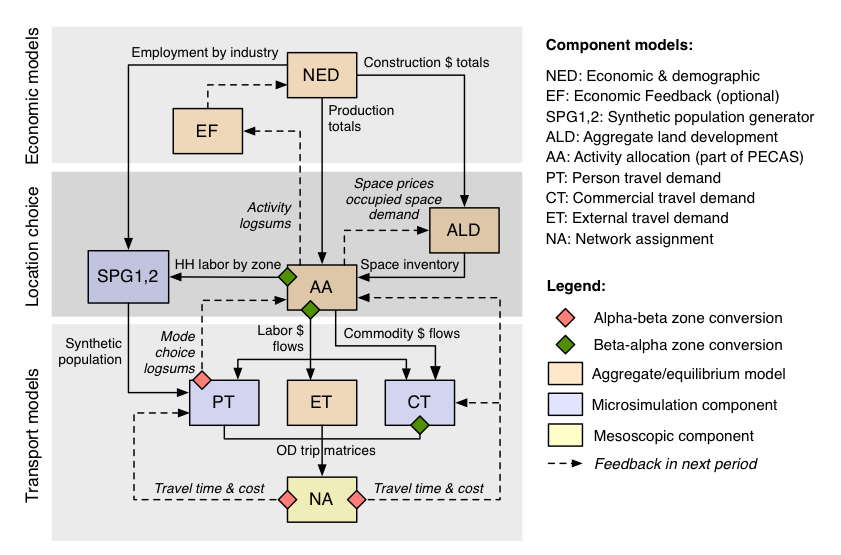
\includegraphics[width=6.0in]{graphics/58-oregon-model-flowchart}
\caption{Oregon statewide model flowchart}
\label{fig:oregon-flowchart}
\end{figure}

\begin{itemize}
\item
The New Economics and Demographics (NED) module determines model-wide production activity levels, employment, and imports and exports based on official Oregon state forecasts. This model is an aggregate formulation, and capable of producing different economic futures.
\item
The Synthetic Population Generator (SPG) module samples household and person demo- graphic attributes (SPG1), and subsequently assigns the household to an alpha zone (SPG2).
\item
The Aggregate Land Development (ALD) module allocates model-wide land development decisions to alpha zones considering floorspace prices and vacancy rates.
\item
The Activity Allocations (AA) module generates production and consumption flows of land (floorspace), labor, and commodities at the beta zone level. It includes the commodity (goods, services, floorspace, and labor) quantities and prices in all exchange zones to clear markets, including the location of businesses and households by beta zone.
\item
The Person Travel (PT) module generates activity-based person trips for each person in the synthetic population during a typical weekday and assigns a workplace by alpha zone. It includes both short and long-distance travel flows, which are combined with commercial vehicle flows in a trip list for traffic assignment.
\item
The Commercial Transport (CT) module maps inter-regional commodity flows into daily truckload equivalents, both within the modeled area and between it and external markets. It also generates internal (to the modeled area) truck tours using a microsimulation framework, to include trips made through distribution centers and intermodal drayage.
\end{itemize}

The roadway and transit network assignments are carried out using the third-party VISUM package for four periods of the day. Still under development is an economic feedback (EF) module, which is a simplified dynamic feedback that adjusts the NED modules fixed model-wide economic forecast, considering the statewide composite location utilities by industry from the AA module.

The SWIM2 system was calibrated and implemented in a staged manner. The preparation and testing of the software code, preparation of validation and calibration data and targets, and estimation and calibration of initial parameters were completed first. The cross-sectional calibration and validation of the full model system (i.e., modules working together) were then carried out. Finally, the system was run through time, subjecting it different policies and stressors (e.g., the introduction of tolling, Interstate highway bridge collapse). A lack of data precluded backcasting. Thus, reasonability checks and stress testing was carried out as part of the final model acceptance testing. The full documentation of the statewide model is published in \cite{donnelly17}.

The design of the activity allocation (AA) module changed over the course of developing the SWIM2 platform. It started out as a microsimulation model, but slowly moved towards an aggregate equilibrium formulation that was inspired, in part, by the MEPLAN model \citep{echenique07}. It later evolved into the Production-Exchange-Consumption Allocation System (PECAS), development of which was undertaken in several places in addition to Oregon \citep{hunt05}. As such, it is fair to describe TLUMIP as an incubator of innovative ideas to model land use changes, having already supported the initial development of UrbanSim.

The SWIM2 development started with traditional multi-year contracting, with a comprehensive model design at the outset. This was the typical approach to large-scale model development in the 1990s, when TLUMIP was launched. Later experiences, and failures in some cases, led to the adoption of the agile development practices becoming more commonly used today. It is a concept from software development that proposes to start with, ``the simplest thing that can possibly work.'' The components are then incrementally developed based upon user and client feedback, continual review of requirements, and performance testing. 

Oregon has benefited from using this approach, despite adopting it while SWIM2 was in development. The questions asked by ODOT stakeholders changed while the program was in motion, and the team shifted development and implementation priorities to accommodate them. This would have required contract amendments and considerable delay had the work been traditionally structured, with deliverables and tasks defined up front.

\subsection{Major applications and implementation}

The first and second-generation models have been used in a variety of studies, but arguably none as important as the Oregon DOT's Bridge Limitations Study. A design flaw was discovered in 2003 that increased the risk of premature cracking in several dozen bridges across the state. The potential repair costs substantially exceeded the agency's budget. However, not addressing them would have resulted in weight restrictions or closures. 

ODOT's modeling staff proposed to the Department's management that the problem should be couched as a community connectivity and economic impact analysis, rather than engineering design issue. It was thought that the legislature would be more receptive if the problem was defined in terms they more quickly understood the implications of. The statewide model was used to test a variety of prioritization packages and effects of bridge limitations. A \$4.3 billion program was approved, in part because of the analyses presented to policy-makers. Moreover, it resulted in prioritizing repairs for communities most affected by loss of connectivity and jobs, rather than the initial assumption that Interstate highway bridges should be addressed first.

The model has also been used in a freight bottleneck study, and is currently being used as part of the Department's ``rough roads'' assessment. The latter focuses on the implications of inadequate maintenance of existing roadway infrastructure across the state. It has the potential to be as important to the Department as the bridge limitations study, and equally well suited for analyses of economic and social impacts.

ODOT has invested \$9.1 million in consultant fees over the course of the program. However, less than a third of this amount has been devoted to the development of the first and second generation models themselves. A larger amount has been spent on data development, to include travel surveys, acquisition of third-party data (including other government agencies), and a commodity flow survey jointly undertaken with Portland Metro and the Port of Portland. Several applications of the model were carried out, both for model acceptance testing and the major studies described above. In addition, two ODOT staff members have been involved for at least half of their time in model design, development, and implementation over the entire period that TLUMIP has been active.

A final key to the success of the SWIM2 system was an active international peer review panel. They have frequently met since the beginning of TLUMIP to oversee model development, envision future revisions and extensions, and to present the latest research conducted at universities and in industry.

\subsection{Lessons learned from Oregon}

Most states have neither the need nor resources to develop as sophisticated a modeling system as Oregon. However, many of the important lessons learned apply to states with less ambitious goals. Some of the key findings from Oregon include:

\begin{itemize}
\item
The questions that policy-makers are facing are changing faster than models used to inform them. The key requirements changed not just once, but twice over the lifespan of TLUMIP, suggesting the need for a more flexible and quickly adaptive modeling framework than typically found in practice.
\item
Along the same lines, the analytical requirements dictated what Oregon wanted to accomplish, rather than simply desiring to have ``better models'' or pursue the state of the art. Their continual re-examination of priorities of decision-makers has required shifting focus several times, but has kept their work relevant to their clients. Oregon would not likely have invested in such a sophisticated modeling system without such requirements. The reminder that applications should dictate design rather than the other way around is a lesson worth repeatedly learning, and has been key to sustained support for their program.
\item
The agile development process is a far better framework for the development of major new platforms than the traditional ``big design up front,'' followed by several years of data and model development. Requirements change over time, new data and methods become available, and experience with interim products often dictate small but important changes in the modeling system that better address the needs of statewide modelers and their clients.
\item
The ability to model freight, their economic linkages, and visualize truck flow patterns is as important, and perhaps more so, than modeling person travel flows. Most of the major applications of the model to date have involved freight, either wholly or in part.
\end{itemize}

The work in Oregon remains a work in progress, and perhaps will always do so. The constantly changing policy environment, the level of questions posed by decision-makers, their zeal for pushing the envelope in land use-transport modeling, and upper management support ensures that they will remain at the forefront of statewide modeling. The investment they have made in their staff is particularly evident, giving them the ability to do many things that many agencies cannot.
